% !TEX TS-program = pdflatex
% !TEX encoding = UTF-8 Unicode

\documentclass[a4paper, titlepage=false, parskip=full-, 10pt]{scrartcl}

\usepackage[utf8]{inputenc}
\usepackage[T1]{fontenc}
\usepackage[english, ngerman]{babel}
\usepackage{babelbib}
\usepackage{hyperref}
\usepackage{listings}
\usepackage{framed}
\usepackage{color}
\usepackage{graphicx}
\usepackage[normalem]{ulem}
\usepackage{cancel}
\usepackage{amsmath}
\usepackage{amssymb}
\usepackage{amsthm}
\usepackage{algorithm}
\usepackage{algorithmic}
\usepackage{geometry}
\usepackage{subfigure}
\geometry{a4paper, top=20mm, left=35mm, right=25mm, bottom=40mm}

\newcounter{tasknbr}
\setcounter{tasknbr}{1}
\newenvironment{task}[1]{{\bf Aufgabe \arabic {tasknbr}\stepcounter{tasknbr}} (#1):\begin{enumerate}}{\end{enumerate}}
\newcommand{\subtask}[1]{\item[#1)]}

% Listings -----------------------------------------------------------------------------
\definecolor{red}{rgb}{.8,.1,.2}
\definecolor{blue}{rgb}{.2,.3,.7}
\definecolor{lightyellow}{rgb}{1.,1.,.97}
\definecolor{gray}{rgb}{.7,.7,.7}
\definecolor{darkgreen}{rgb}{0,.5,.1}
\definecolor{darkyellow}{rgb}{1.,.7,.3}
\lstloadlanguages{C++,[Objective]C,Java}
\lstset{
escapeinside={§§}{§§},
basicstyle=\ttfamily\footnotesize\mdseries,
columns=fullflexible,
keywordstyle=\bfseries\color{blue},
commentstyle=\color{darkgreen},      
stringstyle=\color{red},
numbers=left,
numberstyle=\ttfamily\scriptsize\color{gray},
breaklines=true,
showstringspaces=false,
tabsize=4,
captionpos=b,
float=htb,
frame=tb,
frameshape={RYR}{y}{y}{RYR},
rulecolor=\color{black},
xleftmargin=15pt,
xrightmargin=4pt,
aboveskip=\bigskipamount,
belowskip=\bigskipamount,
backgroundcolor=\color{lightyellow},
extendedchars=true,
belowcaptionskip=15pt}

%% Enter current values here: %%
\newcommand{\lecture}{Robotik WS15/16}
\newcommand{\tutor}{}
\newcommand{\assignmentnbr}{2}
\newcommand{\students}{Julius Auer}
%%-------------------------------------%%

\begin{document}  
{\small \textsl{\lecture \hfill \tutor}}
\hrule
\begin{center}
\textbf{Übungsblatt \assignmentnbr}\\
[\bigskipamount]
{\small \students}
\end{center}
\hrule

\begin{task}{}
\item[]
Annahmen:\\
(A1): Die roten Pfeile kennzeichnen Ursprung und Achsen des Weltkoordinatensystems\\
(A2): Der ''Kasten'' soll im Weltkoordinatensystem fest sein\\
(A3): Die Joints sind Punktförmig

Dürfte wohl so gemeint sein (?).

\subtask{a}
$\Theta_1$ öffnet sich cw und fließt somit mit negativem Vorzeichen in die Rechnung ein. $\Theta_2$ öffnet sich ccw und ist somit positiv. Es ergeben sich die folgenden homogenen Transformations-Matrizen:
\begin{align*}
\begin{pmatrix}x_1\\y_1\end{pmatrix}&=\begin{pmatrix}cos(-\Theta_1)&-sin(-\Theta_1)\\sin(-\Theta_1)&cos(-\Theta_1)\end{pmatrix}\cdot\begin{pmatrix}L_1\\0\end{pmatrix}\\
\begin{pmatrix}x_2\\y_2\\1\end{pmatrix}&=\begin{pmatrix}cos(-\Theta_1)&-sin(-\Theta_1)&0\\sin(-\Theta_1)&cos(-\Theta_1)&0\\0&0&1\end{pmatrix}\cdot\begin{pmatrix}cos(\Theta_2)&-sin(\Theta_2)&L_1\\sin(\Theta_2)&cos(\Theta_2)&0\\0&0&1\end{pmatrix}\cdot\begin{pmatrix}L_2\\0\\1\end{pmatrix}\\
\end{align*}
Oder kompakt:
\begin{align*}
\begin{pmatrix}x_1\\y_1\end{pmatrix}&=\begin{pmatrix}L_1\cdot cos(-\Theta_1)\\L_1\cdot sin(-\Theta_1)\end{pmatrix}\\
\begin{pmatrix}x_2\\y_2\\1\end{pmatrix}&=\begin{pmatrix}L_2\cdot cos(-\Theta_1)\cdot cos(\Theta_2)+L_1\cdot cos(-\Theta_1)-L_2\cdot sin(-\Theta_1)\cdot sin(\Theta_2)\\L_2\cdot sin(-\Theta_1)\cdot cos(\Theta_2)+L_1\cdot sin(-\Theta_1)+L_2\cdot cos(-\Theta_1)\cdot sin(\Theta_2)\\1\end{pmatrix}
\end{align*}

\subtask{b}
\begin{align*}
\frac{\Delta}{\Delta\Theta_1}\begin{pmatrix}x_1\\y_1\end{pmatrix}&=\begin{pmatrix}L_1\cdot sin(-\Theta_1)\\-L_1\cdot cos(-\Theta_1)\end{pmatrix}\\
\frac{\Delta}{\Delta\Theta_2}\begin{pmatrix}x_1\\y_1\end{pmatrix}&=\begin{pmatrix}0\\0\end{pmatrix}\\
\frac{\Delta}{\Delta\Theta_1}\begin{pmatrix}x_2\\y_2\\1\end{pmatrix}&=\begin{pmatrix}L_2\cdot sin(-\Theta_1)\cdot cos(\Theta_2)+L_1\cdot sin(-\Theta_1)+L_2\cdot cos(-\Theta_1)\cdot sin(\Theta_2)\\-L_2\cdot cos(-\Theta_1)\cdot cos(\Theta_2)-L_1\cdot cos(-\Theta_1)+L_2\cdot sin(-\Theta_1)\cdot sin(\Theta_2)\\0\end{pmatrix}\\
\frac{\Delta}{\Delta\Theta_2}\begin{pmatrix}x_2\\y_2\\1\end{pmatrix}&=\begin{pmatrix}-L_2\cdot cos(-\Theta_1)\cdot sin(\Theta_2)-L_2\cdot sin(-\Theta_1)\cdot cos(\Theta_2)\\-L_2\cdot sin(-\Theta_1)\cdot sin(\Theta_2)+L_2\cdot cos(-\Theta_1)\cdot cos(\Theta_2)\\0\end{pmatrix}
\end{align*}
\end{task}

\newpage
\begin{task}{}
\subtask{a}
Äähhmm... dieser Roboter vertritt \emph{keine} politsche Meinung - eigentlich sollte er lediglich winken.

\begin{figure}[htpb]
\begin{center}
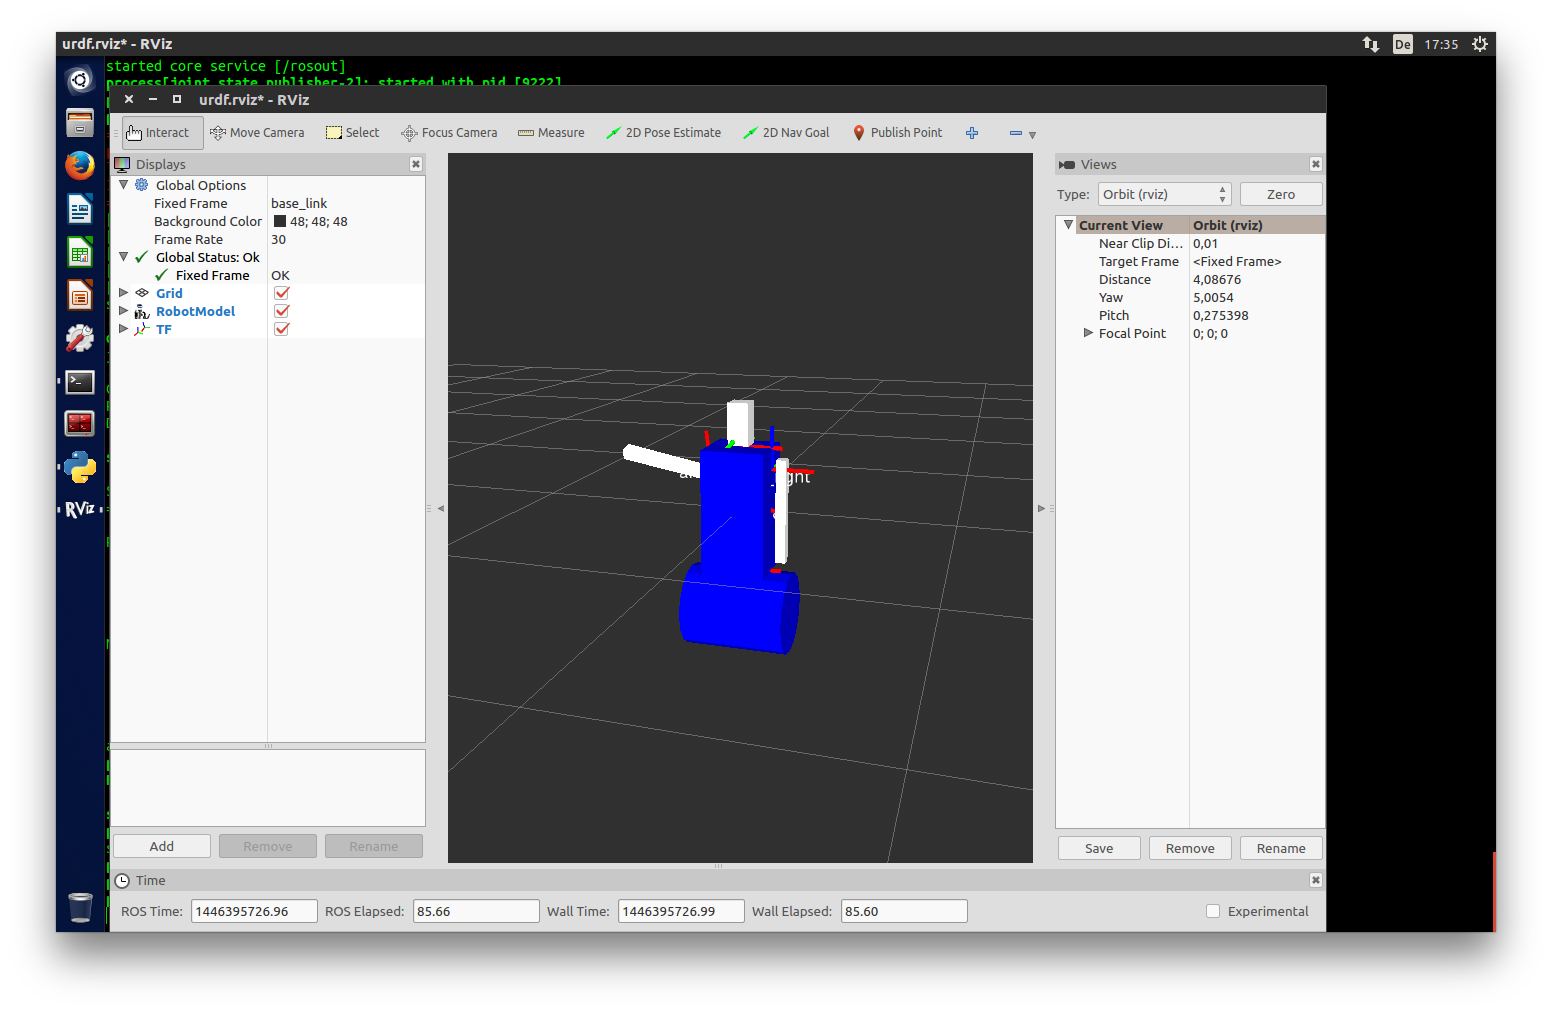
\includegraphics[width=16cm]{capture1.png}
\end{center}
\caption{Mit xacro erstelltes Modell}
\end{figure}

\newpage
\subtask{b}
Naja, \emph{relativ} zum 1. Gelenk hat das 2. Gelenk immer die Koordinaten $\begin{pmatrix}0\\0\\10\end{pmatrix}$. In Weltkoordinaten hat das 2. Gelenk bei der in \emph{c} abgebildeten Pose die Koordinaten $\begin{pmatrix}0\\0.65\\0.76\end{pmatrix}$.

\subtask{c}
\begin{figure}[htpb]
\begin{center}
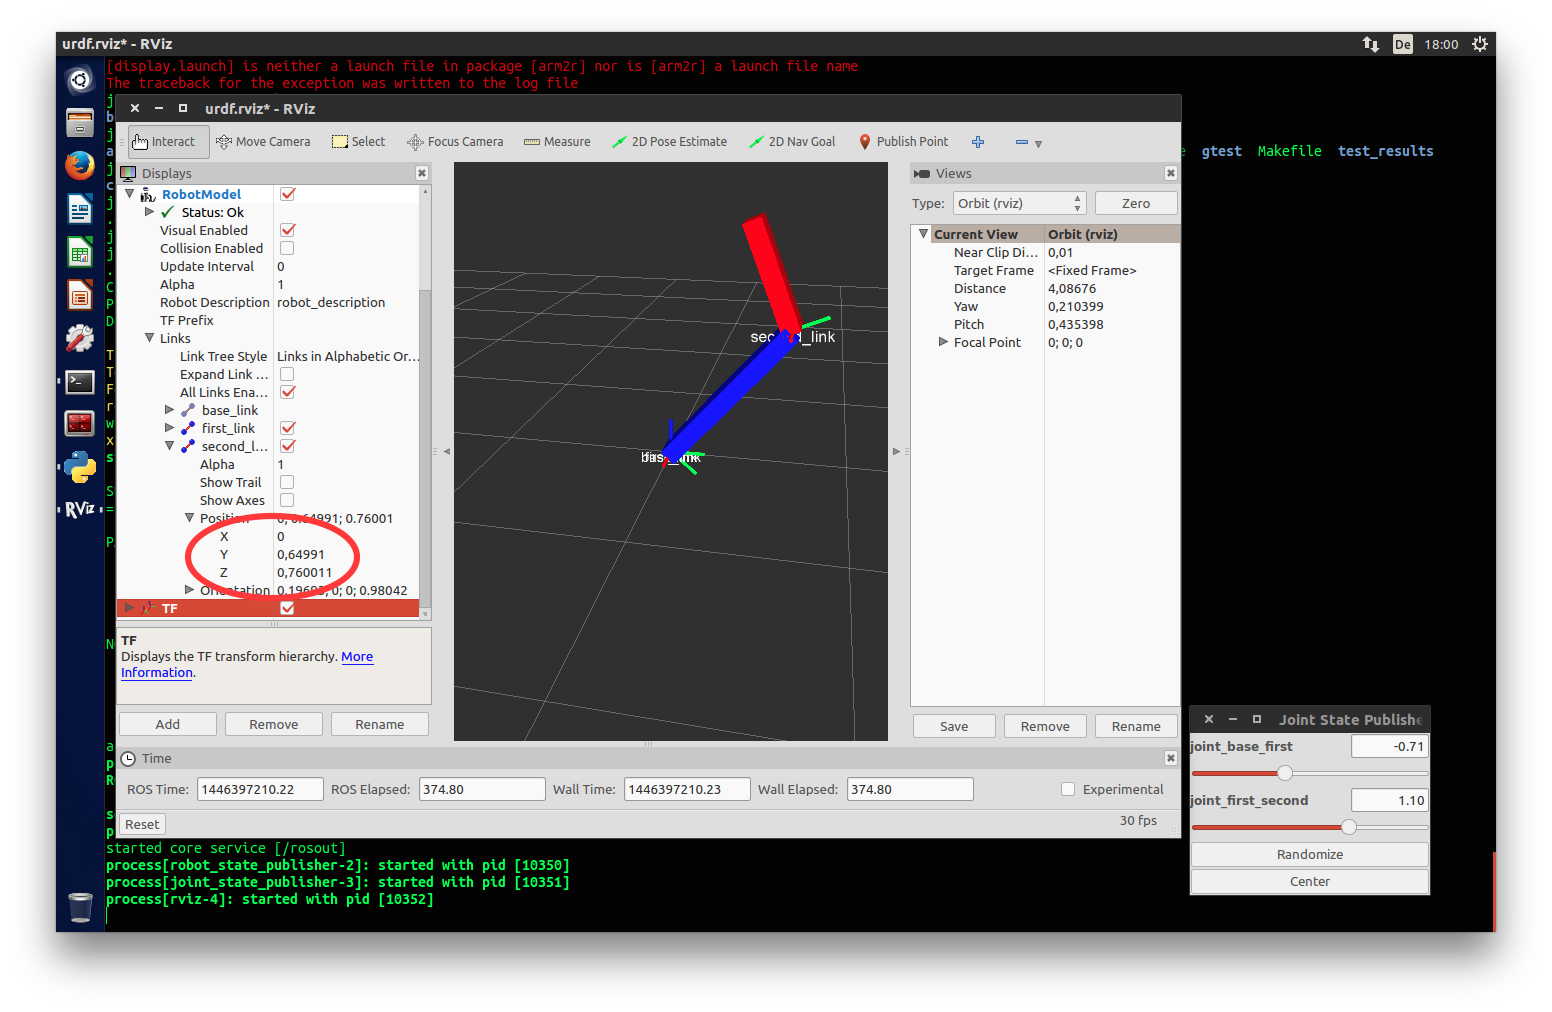
\includegraphics[width=16cm]{capture2.png}
\end{center}
\caption{Pose für arm2r}
\end{figure}
\end{task}
\end{document}